% ============================================================================
% KAPITEL 4: IMPLEMENTATION
% ============================================================================

\chapter{Implementation und technische Umsetzung}
\label{ch:implementation}

\section{Software-Architektur}

Die Implementierung folgt einer modularen Architektur mit 12 spezialisierten Komponenten:

\begin{figure}[htbp]
\centering
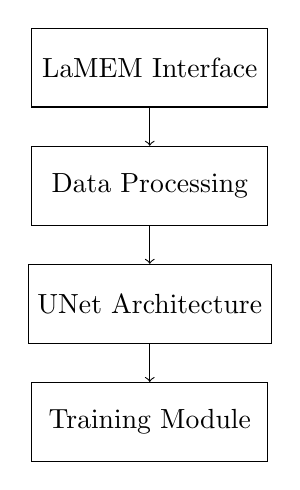
\begin{tikzpicture}[
    node distance=1.5cm,
    box/.style={rectangle, draw, minimum width=3cm, minimum height=1cm}
]
    % Nodes
    \node[box] (lamem) {LaMEM Interface};
    \node[box, below of=lamem] (data) {Data Processing};
    \node[box, below of=data] (unet) {UNet Architecture};
    \node[box, below of=unet] (train) {Training Module};
    
    % Arrows
    \draw[->] (lamem) -- (data);
    \draw[->] (data) -- (unet);
    \draw[->] (unet) -- (train);
\end{tikzpicture}
\caption{Modulare Software-Architektur}
\label{fig:architecture}
\end{figure}

\section{Technische Herausforderungen}

\subsection{Zygote-Kompatibilität}

Die ursprüngliche Implementierung verwendete mutating Array-Operationen, die mit Zygote.jl inkompatibel sind:

\begin{lstlisting}[language=Julia, caption={Problem: Mutating Arrays}]
# Zygote-inkompatibel
function forward_pass(x)
    skip_features = []
    push!(skip_features, x)  # Mutation!
end
\end{lstlisting}

\begin{lstlisting}[language=Julia, caption={Lösung: Immutable Operations}]
# Zygote-kompatibel
function forward_pass(x)
    skip_features = (x,)  # Tuple statt Array
end
\end{lstlisting}

\subsection{GPU-Memory Management}

Adaptive Batch-Größen basierend auf verfügbarem GPU-Speicher:

\begin{table}[htbp]
\centering
\caption{Optimale Batch-Größen nach Auflösung}
\label{tab:batch_sizes}
\begin{tabular}{@{}cc@{}}
\toprule
\textbf{Auflösung} & \textbf{Max. Batch-Größe} \\
\midrule
64×64 & 16 \\
128×128 & 8 \\
256×256 & 4 \\
512×512 & 1 \\
\bottomrule
\end{tabular}
\end{table}